\pdfoutput=1
\documentclass[11pt]{article}

% Supplementary appendix to paper.tex. Compile separately (pdflatex appendix.tex).
% All tables under appendix/tables/ and the figure under appendix/figures/ are generated by
% scripts/make_appendix.py from results/; rerun it instead of editing them by hand.
\usepackage{EACL2023}

\usepackage{times}
\usepackage{latexsym}
\usepackage[T1]{fontenc}
\usepackage[utf8]{inputenc}
\usepackage{microtype}
\usepackage{inconsolata}
\usepackage{booktabs}
\usepackage{longtable}
\usepackage{graphicx}
\usepackage{amsmath}
\usepackage{amssymb}

\newcommand{\Cd}{C_{\mathrm{desc}}}
\renewcommand{\thesection}{\Alph{section}}
\renewcommand{\thetable}{\thesection.\arabic{table}}
\renewcommand{\thefigure}{\thesection.\arabic{figure}}
\makeatletter\@addtoreset{table}{section}\@addtoreset{figure}{section}\makeatother

\begin{document}
% The ACL \maketitle switches to two columns, which longtable cannot use; one-column title instead.
\onecolumn
\begin{center}
{\Large\bfseries Supplementary Appendix to ``Noise in Disguise:\\[2pt]
What Powers Physics-Inspired GNN Colouring''\par}
\vspace{1em}
{\large Semyon Guretskiy (336249255) \quad Ori Petel (325211498) \quad Adi Shimoni (316342435)\par}
\vspace{1.5em}
\end{center}

\noindent This appendix gives the experimental details and the full results behind every number
in the main paper. Section~\ref{sec:setup} describes the setup, Sections~\ref{sec:rq1}--\ref{sec:rq3}
give the complete comparisons for each research question, Section~\ref{sec:pergraph} lists
per-graph results, and Section~\ref{sec:sdp} reports a further effort with domain knowledge. The
tables of Sections~\ref{sec:setup}--\ref{sec:pergraph} are generated from the stored results by one
script (\texttt{scripts/make\_appendix.py}); references to ``Table~$n$'' without a letter are to the
main paper.

\section{Experimental setup}
\label{sec:setup}

\paragraph{Benchmark and regime.} We use the 68 DIMACS colouring graphs whose chromatic number is
proven and at least 3 (11 to 1{,}000 vertices, 14 families; Table~\ref{tab:pergraph}). Every run uses
$k=\chi-1$ colours, so zero conflicts are impossible and every method is compared on a graded conflict
count. Each method runs 5 seeds (0--4) per graph. Unless stated otherwise, results are at exactly
$10^5$ full-batch steps; there is no early stopping and no best-checkpoint selection.

\paragraph{Models and tuning.} Table~\ref{tab:hparams} lists the selected settings. A, B, C and D are
tuned separately with the same two-stage random search on 13 synthetic graphs disjoint from the
benchmark (Erd\H{o}s--R\'enyi, Watts--Strogatz, random-regular and planted instances), at palettes
$k=\chi_{\mathrm{hi}}$ and $\chi_{\mathrm{hi}}-1$. Stage~1 evaluates 43 configurations (3 references
and 40 random draws; 2 seeds, $10^4$ steps); stage~2 evaluates the top 6 plus 4 new draws (3 seeds,
$5{\cdot}10^4$ steps). The score is the mean rank of seed-averaged final argmax conflicts, so tuning
does not select for the after-descent metric. B-rand and the noisy B arms reuse B's settings;
A-no-drop reuses A's settings with dropout set to 0 (not retuned). The noise levels
$\sigma\in\{0.5,1,2\}$ were fixed before their comparison and were not tuned.

\begin{table}[h]
\centering\small
\begin{tabular}{@{}lllccc@{}}
\toprule
arm & optimiser & learning rate & embedding / hidden width & dropout & weight decay \\
\midrule
A (PI-GNN) & AdamW & 0.0196 & 85 / 30 & 0.466 & 0.01 \\
A-no-drop & AdamW & 0.0196 & 85 / 30 & 0 & 0.01 \\
B, B-rand, B-noise-$\sigma$ & AdamW & 0.0427 & direct $n\times k$ logits & 0 & 0.0639 \\
C (node MLP) & AdamW & 0.0281 & 55 / 39 & 0.202 & 0.01 \\
D (linearised) & Adam & 0.00216 & A's initial network and Jacobian & 0 & 0 \\
\bottomrule
\end{tabular}
\caption{Selected hyperparameters (from \texttt{configs/*\_frozen.json}). A uses two mean-aggregation
GraphSAGE layers with ReLU; C uses the same layers without the neighbour terms. Dropout is active only
during training.}
\label{tab:hparams}
\end{table}

\paragraph{Arms.} B optimises the logit matrix $Z$ directly, initialised at A's exact initial output
$Z_0$; B-rand starts from scale-matched random logits instead. B-noise-$\sigma$ trains on
$\mathrm{softmax}(Z+\sigma\varepsilon)$ with fresh $\varepsilon\sim N(0,I)$ at every step and is always
evaluated on clean $Z$. C removes the neighbour terms from both SAGE layers. D trains
$Z(\delta)=Z_0+J_0\delta$ with A's Jacobian $J_0$ at initialisation frozen, implemented with
Jacobian--vector products.

\paragraph{Budgets and time matching.} For B, B-rand, the noisy B arms and D, an extra checkpoint is
saved at the first step whose cumulative training time reaches A's $10^5$-step training time on the
same graph and seed (``time'' rows in Table~\ref{tab:rq2all}). At that point B has taken a median of
about $2.9\times10^5$ steps and D about $8.3\times10^4$. A-no-drop and C have matched-step results only.
Runs used shared TITAN Xp and RTX~2080~Ti GPUs, so time matching is approximate.

\paragraph{Repair and decoders.} \emph{Strict descent} repeatedly recolours a vertex with the largest
positive gain $\gamma_v$ (seeded random tie-breaking) and stops at a single-flip optimal (SFO)
colouring; it never takes neutral or worsening moves. \emph{D-CE} fixes vertices in DSATUR order
(most distinct colours among fixed neighbours, then degree, then index) and gives each the colour
minimising fixed-neighbour conflicts plus $\sum_u p_u(a)$ over unfixed neighbours; on exactly uniform
$P$ it equals fixed-$k$ DSATUR (unit-tested). The \emph{near-uniform} input is
$\mathrm{softmax}(0.1\,\Xi)$ with $\Xi_{v,a}\sim N(0,1)$. \emph{Colour-scrambled} permutes the colour
coordinates of each row independently; \emph{vertex-shuffled} permutes rows across vertices;
\emph{untrained} is the softmax of A's initial logits. Sampling draws 32 colourings from $P$, repairs
each and keeps the best. Every decoded colouring receives the same strict descent.

\paragraph{TabuCol.} Galinier--Hao TabuCol with tenure $L+\lfloor0.6\,|\text{conflicted}|\rfloor$,
$L\sim U\{0,\dots,9\}$, aspiration, and random tie-breaking; 10 seeds per graph; wall-clock budget
equal to PI-GNN's mean $10^5$-step training time on that graph. It returns the best colouring seen.

\paragraph{Statistics.} The graph is the unit of analysis. For each graph we average the seeds of
both methods and compute $d_g=(X_g-Y_g)/\max(Y_g,1)$ (negative favours the first method). A graph is
a practical tie if $|X_g-Y_g|<1$ or $|d_g|\le5\%$, otherwise a win or loss (W/T/L). $p$ is a two-sided
Wilcoxon signed-rank test on the nonzero $d_g$; it is descriptive except for the primary comparisons.
\textbf{The 95\% confidence intervals} reported here, which the main paper omits, are percentile
bootstrap intervals for the median $d_g$, resampling the 68 graphs with replacement (10{,}000
resamples). They treat the benchmark graphs as exchangeable, which DIMACS is not, so they describe
the uncertainty of the benchmark summary rather than a population of graphs. Means give each graph
equal weight and are dominated by a few dense graphs.

\section{RQ1: what training produces}
\label{sec:rq1}

\begin{table}[h]
\centering\small
% generated by scripts/make_appendix.py -- do not edit by hand
\begin{tabular}{@{}rrrrrr@{}}
\toprule
step & SFO runs (\%) & removable by descent (\%) & mean raw $C$ & mean $\Cd$ & mean entropy \\
\midrule
1 & 0.0 & 94.9 & 1267.3 & 132.1 & 1.81 \\
2 & 0.6 & 92.8 & 913.3 & 132.3 & 1.83 \\
5 & 0.3 & 91.3 & 794.0 & 133.6 & 1.76 \\
10 & 0.6 & 87.1 & 656.2 & 131.7 & 1.63 \\
20 & 1.8 & 83.9 & 1247.8 & 132.8 & 1.42 \\
50 & 2.6 & 72.4 & 6170.1 & 130.4 & 0.994 \\
100 & 4.4 & 61.5 & 5544.6 & 129.6 & 0.679 \\
200 & 9.4 & 45.9 & 4662.6 & 129.7 & 0.52 \\
500 & 18.2 & 36.6 & 3765.4 & 128.1 & 0.411 \\
1{,}000 & 24.4 & 28.3 & 2908.2 & 128.8 & 0.336 \\
2{,}000 & 28.5 & 27.3 & 2764.8 & 127.6 & 0.281 \\
5{,}000 & 30.6 & 25.9 & 2927.8 & 125.3 & 0.257 \\
10{,}000 & 32.1 & 18.9 & 2558.9 & 123.9 & 0.284 \\
20{,}000 & 35.0 & 15.6 & 2541.8 & 122.5 & 0.337 \\
50{,}000 & 37.9 & 10.4 & 2063.2 & 118.7 & 0.31 \\
100{,}000 & 42.1 & 10.5 & 1517.3 & 114.9 & 0.256 \\
\bottomrule
\end{tabular}

\caption{PI-GNN's argmax output over training (68 graphs, 5 seeds; the data of Figure~2). SFO: share
of the 340 runs that are single-flip optimal. Removable: median over graphs of the share of raw
conflicts that strict descent removes.}
\label{tab:rq1traj}
\end{table}

\begin{table}[h]
\centering\small
% generated by scripts/make_appendix.py -- do not edit by hand
\begin{tabular}{@{}lccccr@{}}
\toprule
Comparison (first vs.\ second) & W/T/L & median $d$ & 95\% CI & mean $C$, first / second & $p$ \\
\midrule
PI-GNN vs.\ random colouring & 62/5/1 & $-38.7\%$ & [$-48.2\%$, $-28.0\%$] & 114.9 / 134.5 & $5.1{\times}10^{-12}$ \\
PI-GNN vs.\ own epoch-1 output & 59/8/1 & $-32.5\%$ & [$-43.9\%$, $-23.2\%$] & 114.9 / 132.1 & $2.1{\times}10^{-12}$ \\
PI-GNN vs.\ DSATUR (fixed $k$) & 16/28/24 & $0.0\%$ & [$0.0\%$, $+13.1\%$] & 114.9 / 121.9 & 0.003 \\
PI-GNN vs.\ DSATUR, random ties & 29/24/15 & $-5.2\%$ & [$-11.5\%$, $0.0\%$] & 114.9 / 120.7 & 0.617 \\
PI-GNN vs.\ DSATUR, random vertex ties & 19/26/23 & $0.0\%$ & [$-1.1\%$, $+10.4\%$] & 114.9 / 116.1 & 0.006 \\
PI-GNN + desc.\ vs.\ TabuCol (time-matched) & 14/13/41 & $+45.3\%$ & [$+7.6\%$, $+80.6\%$] & 114.9 / 70.4 & $1.6{\times}10^{-4}$ \\
PI-GNN raw vs.\ TabuCol (time-matched) & 11/11/46 & $+80.0\%$ & [$+44.8\%$, $+175.5\%$] & 1517.3 / 70.4 & $6.4{\times}10^{-8}$ \\
\bottomrule
\end{tabular}

\caption{PI-GNN + descent at $10^5$ steps against starts given the same descent, and against TabuCol
(Table~1 with confidence intervals and the exploratory DSATUR tie-breaking variants). Negative $d$
favours PI-GNN; the TabuCol medians quantify the gap that Table~1 reports only as W/T/L.}
\label{tab:rq1ctrl}
\end{table}

\noindent\textbf{Confidence at $10^5$ steps.} % generated by scripts/make_appendix.py -- do not edit by hand
median graph: 99.66\% of vertices with $p_{\max}\ge0.99$, median top-two logit gap 205; improvable vertices (graphs with any, 51): 100\% above 0.99, gap 149
\unskip.
Statistics for improvable vertices average only runs that have one.

\begin{table}[h]
\centering\small
% generated by scripts/make_appendix.py -- do not edit by hand
\begin{tabular}{@{}lrrrrcc@{}}
\toprule
family & graphs & SFO runs (\%) & median improvable & confident (\%) & vs.\ DSATUR & vs.\ TabuCol \\
\midrule
Queen & 12 & 85 & 0.0 & 100.0 & 8/3/1 & 0/0/12 \\
DSJC & 4 & 45 & 31.5 & 99.3 & 2/1/1 & 0/0/4 \\
School & 2 & 0 & 7.5 & 99.8 & 1/0/1 & 0/0/2 \\
Flat & 5 & 0 & 20.0 & 99.8 & 1/4/0 & 0/0/5 \\
Leighton & 12 & 38 & 1.0 & 99.9 & 4/3/5 & 0/0/12 \\
DSJR & 3 & 33 & 450.0 & 34.6 & 0/0/3 & 0/0/3 \\
fpsol & 3 & 0 & 18.0 & 98.7 & 0/0/3 & 3/0/0 \\
inithx & 3 & 0 & 27.0 & 98.5 & 0/0/3 & 3/0/0 \\
Miles & 5 & 24 & 16.0 & 99.2 & 0/1/4 & 0/2/3 \\
zeroin & 3 & 0 & 14.0 & 99.0 & 0/1/2 & 3/0/0 \\
mulsol & 5 & 8 & 8.0 & 99.2 & 0/5/0 & 5/0/0 \\
Mycielski & 5 & 84 & 0.0 & 99.6 & 0/5/0 & 0/5/0 \\
Social (book) & 5 & 84 & 0.0 & 98.6 & 0/4/1 & 0/5/0 \\
games120 & 1 & 100 & 0.0 & 99.5 & 0/1/0 & 0/1/0 \\
\bottomrule
\end{tabular}

\caption{RQ1 by family at $10^5$ steps. SFO runs: share of the family's runs that are single-flip
optimal. Median improvable: improvable vertices per run (median over runs). Confident: median over
graphs of the share of vertices with $p_{\max}\ge0.99$. The last two columns are W/T/L from
PI-GNN's side (PI-GNN better / tie / reference better) after descent.}
\label{tab:rq1fam}
\end{table}

\section{RQ2: is the network needed?}
\label{sec:rq2}

\begin{table}[h]
\centering\small
% generated by scripts/make_appendix.py -- do not edit by hand
\begin{tabular}{@{}lrrrrrr@{}}
\toprule
arm & SFO runs (\%) & mean raw $C$ & mean $\Cd$ & confident (\%) & logit gap & entropy \\
\midrule
A (PI-GNN) & 42 & 1517.3 & 114.9 & 99.6 & 203.7 & 0.00099 \\
A-no-drop & 17 & 1558.4 & 115.7 & 97.9 & 17.9 & 0.0081 \\
C (MLP) & 41 & 133.1 & 120.4 & 99.9 & 138.5 & 0.00033 \\
D (linearised) & 42 & 172.6 & 130.4 & 96.9 & 23.4 & 0.017 \\
B & 100 & 108.6 & 108.6 & 100.0 & 18.4 & 0.00014 \\
B-rand & 100 & 107.1 & 107.1 & 100.0 & 18.5 & 0.00016 \\
B-noise-0.5 & 100 & 109.2 & 109.2 & 100.0 & 18.6 & 0.00016 \\
B-noise-1 & 100 & 92.5 & 92.5 & 99.7 & 13.0 & 0.0015 \\
B-noise-2 & 100 & 83.4 & 83.4 & 93.2 & 8.3 & 0.047 \\
\bottomrule
\end{tabular}

\caption{Endpoint summary per arm at $10^5$ steps (the SFO and logit-gap columns of Table~2). SFO:
share of the 340 runs. Confident, logit gap (median top-two logit difference) and entropy (mean
row entropy, nats) are medians over graphs of seed means, from clean evaluation logits.}
\label{tab:rq2diag}
\end{table}

% generated by scripts/make_appendix.py -- do not edit by hand
\begin{longtable}{@{}lccccr@{}}
\caption{All RQ2 comparisons at $10^5$ steps (68 graphs, 5 seeds). ``time'': the first arm is evaluated at the
checkpoint whose training time matches A's (or the reference arm's) $10^5$-step time. Rows above the rule are the
three pre-registered primary comparisons; the rest are secondary and descriptive. Negative $d$ favours the first
arm.}\label{tab:rq2all}\\
\toprule
Comparison (first vs.\ second) & W/T/L & median $d$ & 95\% CI & mean $C$, first / second & $p$ \\
\midrule\endfirsthead
\toprule
Comparison (first vs.\ second) & W/T/L & median $d$ & 95\% CI & mean $C$, first / second & $p$ \\
\midrule\endhead
\bottomrule\endfoot
B vs.\ A, raw & 32/23/13 & $-8.6\%$ & [$-22.9\%$, $0.0\%$] & 108.6 / 1517.3 & 0.002 \\
B vs.\ A, desc. & 17/25/26 & $+6.0\%$ & [$0.0\%$, $+20.0\%$] & 108.6 / 114.9 & $7.5{\times}10^{-4}$ \\
B vs.\ A, raw, time & 32/23/13 & $-8.6\%$ & [$-22.9\%$, $0.0\%$] & 108.5 / 1517.3 & 0.002 \\
B vs.\ A, desc., time & 17/26/25 & $+6.0\%$ & [$0.0\%$, $+20.0\%$] & 108.5 / 114.9 & $8.1{\times}10^{-4}$ \\
B vs.\ B-rand, raw & 14/42/12 & $-0.2\%$ & [$-4.9\%$, $+0.3\%$] & 108.6 / 107.1 & 0.020 \\
B vs.\ B-rand, desc. & 14/42/12 & $-0.2\%$ & [$-4.9\%$, $+0.3\%$] & 108.6 / 107.1 & 0.020 \\
\midrule
B-rand vs.\ A, raw & 28/21/19 & $-2.4\%$ & [$-14.3\%$, $+1.8\%$] & 107.1 / 1517.3 & 0.145 \\
B-rand vs.\ A, desc. & 20/20/28 & $+10.8\%$ & [$0.0\%$, $+27.2\%$] & 107.1 / 114.9 & $3.5{\times}10^{-4}$ \\
B-rand vs.\ A, raw, time & 28/21/19 & $-2.4\%$ & [$-14.3\%$, $+1.6\%$] & 106.9 / 1517.3 & 0.145 \\
B-rand vs.\ A, desc., time & 20/20/28 & $+10.8\%$ & [$0.0\%$, $+27.2\%$] & 106.9 / 114.9 & $3.8{\times}10^{-4}$ \\
B vs.\ A-no-drop, raw & 62/5/1 & $-63.3\%$ & [$-73.1\%$, $-56.2\%$] & 108.6 / 1558.4 & $1.4{\times}10^{-12}$ \\
B vs.\ A-no-drop, desc. & 30/23/15 & $-8.0\%$ & [$-11.1\%$, $0.0\%$] & 108.6 / 115.7 & 0.701 \\
A-no-drop vs.\ A, raw & 10/9/49 & $+119.0\%$ & [$+59.0\%$, $+175.7\%$] & 1558.4 / 1517.3 & $4.3{\times}10^{-9}$ \\
A-no-drop vs.\ A, desc. & 7/40/21 & $+8.7\%$ & [$+0.9\%$, $+14.3\%$] & 115.7 / 114.9 & $2.0{\times}10^{-4}$ \\
B-noise-0.5 vs.\ A, raw & 33/21/14 & $-10.9\%$ & [$-23.6\%$, $0.0\%$] & 109.2 / 1517.3 & $4.2{\times}10^{-4}$ \\
B-noise-0.5 vs.\ A, desc. & 20/19/29 & $+5.8\%$ & [$0.0\%$, $+17.4\%$] & 109.2 / 114.9 & 0.002 \\
B-noise-0.5 vs.\ A, raw, time & 33/21/14 & $-10.9\%$ & [$-23.6\%$, $0.0\%$] & 109.2 / 1517.3 & $4.2{\times}10^{-4}$ \\
B-noise-0.5 vs.\ A, desc., time & 20/19/29 & $+5.8\%$ & [$0.0\%$, $+17.4\%$] & 109.2 / 114.9 & 0.002 \\
B-noise-0.5 vs.\ B, raw & 10/55/3 & $-0.8\%$ & [$-2.4\%$, $0.0\%$] & 109.2 / 108.6 & 0.156 \\
B-noise-0.5 vs.\ B, desc. & 10/55/3 & $-0.8\%$ & [$-2.4\%$, $0.0\%$] & 109.2 / 108.6 & 0.156 \\
B-noise-0.5 vs.\ B, raw, time & 10/55/3 & $-0.8\%$ & [$-2.4\%$, $0.0\%$] & 109.2 / 108.5 & 0.162 \\
B-noise-0.5 vs.\ B, desc., time & 10/55/3 & $-0.8\%$ & [$-2.4\%$, $0.0\%$] & 109.2 / 108.5 & 0.162 \\
B-noise-0.5 vs.\ A-no-drop, raw & 62/5/1 & $-63.6\%$ & [$-72.3\%$, $-57.4\%$] & 109.2 / 1558.4 & $1.2{\times}10^{-12}$ \\
B-noise-0.5 vs.\ A-no-drop, desc. & 32/23/13 & $-8.1\%$ & [$-10.6\%$, $0.0\%$] & 109.2 / 115.7 & 0.433 \\
B-noise-1 vs.\ A, raw & 46/20/2 & $-37.7\%$ & [$-46.5\%$, $-22.9\%$] & 92.5 / 1517.3 & $1.5{\times}10^{-10}$ \\
B-noise-1 vs.\ A, desc. & 35/30/3 & $-15.9\%$ & [$-24.5\%$, $-5.4\%$] & 92.5 / 114.9 & $4.0{\times}10^{-7}$ \\
B-noise-1 vs.\ A, raw, time & 49/18/1 & $-44.4\%$ & [$-51.8\%$, $-28.1\%$] & 87.7 / 1517.3 & $2.5{\times}10^{-11}$ \\
B-noise-1 vs.\ A, desc., time & 38/28/2 & $-22.4\%$ & [$-28.7\%$, $-13.4\%$] & 87.7 / 114.9 & $6.3{\times}10^{-9}$ \\
B-noise-1 vs.\ B, raw & 49/19/0 & $-26.9\%$ & [$-36.9\%$, $-19.1\%$] & 92.5 / 108.6 & $1.1{\times}10^{-11}$ \\
B-noise-1 vs.\ B, desc. & 49/19/0 & $-26.9\%$ & [$-36.9\%$, $-19.1\%$] & 92.5 / 108.6 & $1.1{\times}10^{-11}$ \\
B-noise-1 vs.\ B, raw, time & 52/16/0 & $-35.4\%$ & [$-41.6\%$, $-26.2\%$] & 87.7 / 108.5 & $7.6{\times}10^{-12}$ \\
B-noise-1 vs.\ B, desc., time & 52/16/0 & $-35.4\%$ & [$-41.6\%$, $-26.2\%$] & 87.7 / 108.5 & $7.6{\times}10^{-12}$ \\
B-noise-1 vs.\ A-no-drop, raw & 62/6/0 & $-77.1\%$ & [$-83.6\%$, $-69.4\%$] & 92.5 / 1558.4 & $1.1{\times}10^{-12}$ \\
B-noise-1 vs.\ A-no-drop, desc. & 41/26/1 & $-26.0\%$ & [$-31.3\%$, $-20.5\%$] & 92.5 / 115.7 & $4.1{\times}10^{-10}$ \\
B-noise-2 vs.\ A, raw & 53/13/2 & $-48.6\%$ & [$-56.4\%$, $-31.6\%$] & 83.4 / 1517.3 & $1.6{\times}10^{-11}$ \\
B-noise-2 vs.\ A, desc. & 44/21/3 & $-27.5\%$ & [$-33.9\%$, $-15.6\%$] & 83.4 / 114.9 & $1.4{\times}10^{-8}$ \\
B-noise-2 vs.\ A, raw, time & 53/13/2 & $-50.0\%$ & [$-59.6\%$, $-32.0\%$] & 81.6 / 1517.3 & $8.3{\times}10^{-12}$ \\
B-noise-2 vs.\ A, desc., time & 44/21/3 & $-29.1\%$ & [$-38.0\%$, $-17.0\%$] & 81.6 / 114.9 & $4.4{\times}10^{-9}$ \\
B-noise-2 vs.\ B, raw & 53/15/0 & $-39.4\%$ & [$-47.8\%$, $-31.1\%$] & 83.4 / 108.6 & $8.0{\times}10^{-12}$ \\
B-noise-2 vs.\ B, desc. & 53/15/0 & $-39.4\%$ & [$-47.8\%$, $-30.9\%$] & 83.4 / 108.6 & $8.0{\times}10^{-12}$ \\
B-noise-2 vs.\ B, raw, time & 54/14/0 & $-42.7\%$ & [$-50.0\%$, $-33.4\%$] & 81.6 / 108.5 & $7.9{\times}10^{-12}$ \\
B-noise-2 vs.\ B, desc., time & 54/14/0 & $-42.7\%$ & [$-50.0\%$, $-33.4\%$] & 81.6 / 108.5 & $7.9{\times}10^{-12}$ \\
B-noise-2 vs.\ A-no-drop, raw & 64/4/0 & $-81.4\%$ & [$-86.8\%$, $-72.8\%$] & 83.4 / 1558.4 & $1.1{\times}10^{-12}$ \\
B-noise-2 vs.\ A-no-drop, desc. & 45/21/2 & $-32.9\%$ & [$-45.1\%$, $-27.0\%$] & 83.4 / 115.7 & $7.5{\times}10^{-10}$ \\
C vs.\ A, raw & 20/28/20 & $+1.4\%$ & [$-2.5\%$, $+9.8\%$] & 133.1 / 1517.3 & 0.600 \\
C vs.\ A, desc. & 5/35/28 & $+7.8\%$ & [$+2.1\%$, $+16.3\%$] & 120.4 / 114.9 & $5.5{\times}10^{-6}$ \\
C vs.\ B, raw & 4/31/33 & $+9.9\%$ & [$+5.6\%$, $+17.9\%$] & 133.1 / 108.6 & $2.4{\times}10^{-5}$ \\
C vs.\ B, desc. & 10/36/22 & $0.0\%$ & [$-3.5\%$, $+5.8\%$] & 120.4 / 108.6 & 0.994 \\
C vs.\ A-no-drop, raw & 62/3/3 & $-60.1\%$ & [$-71.7\%$, $-51.5\%$] & 133.1 / 1558.4 & $3.1{\times}10^{-10}$ \\
C vs.\ A-no-drop, desc. & 15/39/14 & $0.0\%$ & [$-4.6\%$, $+2.3\%$] & 120.4 / 115.7 & 0.869 \\
D vs.\ A, raw & 14/12/42 & $+31.0\%$ & [$+20.9\%$, $+41.2\%$] & 172.6 / 1517.3 & 0.001 \\
D vs.\ A, desc. & 0/10/58 & $+36.6\%$ & [$+23.4\%$, $+57.9\%$] & 130.4 / 114.9 & $3.5{\times}10^{-12}$ \\
D vs.\ A, raw, time & 14/12/42 & $+29.5\%$ & [$+20.5\%$, $+41.6\%$] & 173.4 / 1517.3 & $5.7{\times}10^{-4}$ \\
D vs.\ A, desc., time & 0/9/59 & $+38.3\%$ & [$+23.3\%$, $+60.4\%$] & 131.2 / 114.9 & $3.5{\times}10^{-12}$ \\
D vs.\ B, raw & 0/9/59 & $+50.8\%$ & [$+39.7\%$, $+66.4\%$] & 172.6 / 108.6 & $3.5{\times}10^{-12}$ \\
D vs.\ B, desc. & 0/15/53 & $+35.8\%$ & [$+25.0\%$, $+43.2\%$] & 130.4 / 108.6 & $6.5{\times}10^{-12}$ \\
D vs.\ B, raw, time & 0/9/59 & $+58.3\%$ & [$+42.9\%$, $+72.7\%$] & 173.4 / 108.5 & $3.5{\times}10^{-12}$ \\
D vs.\ B, desc., time & 0/14/54 & $+42.0\%$ & [$+29.1\%$, $+47.5\%$] & 131.2 / 108.5 & $5.9{\times}10^{-12}$ \\
D vs.\ A-no-drop, raw & 55/7/6 & $-45.6\%$ & [$-56.8\%$, $-34.6\%$] & 172.6 / 1558.4 & $2.3{\times}10^{-9}$ \\
D vs.\ A-no-drop, desc. & 1/15/52 & $+22.7\%$ & [$+13.4\%$, $+30.9\%$] & 130.4 / 115.7 & $9.2{\times}10^{-11}$ \\
\end{longtable}


\begin{table}[h]
\centering\small
% generated by scripts/make_appendix.py -- do not edit by hand
\begin{tabular}{@{}lrcccccc@{}}
\toprule
family & graphs & B vs.\ A & A-no-drop vs.\ A & B-noise-2 vs.\ A & B-noise-2 vs.\ B & C vs.\ A & D vs.\ A \\
\midrule
Queen & 12 & 1/3/8 & 0/0/12 & 10/2/0 & 11/1/0 & 0/4/8 & 0/0/12 \\
DSJC & 4 & 3/0/1 & 1/0/3 & 3/0/1 & 4/0/0 & 1/1/2 & 0/1/3 \\
School & 2 & 2/0/0 & 1/1/0 & 2/0/0 & 2/0/0 & 0/1/1 & 0/0/2 \\
Flat & 5 & 4/1/0 & 0/4/1 & 5/0/0 & 5/0/0 & 0/4/1 & 0/1/4 \\
Leighton & 12 & 3/4/5 & 0/9/3 & 10/1/1 & 11/1/0 & 0/6/6 & 0/0/12 \\
DSJR & 3 & 2/0/1 & 1/1/1 & 3/0/0 & 3/0/0 & 2/0/1 & 0/0/3 \\
fpsol & 3 & 0/0/3 & 1/2/0 & 3/0/0 & 3/0/0 & 0/1/2 & 0/0/3 \\
inithx & 3 & 0/0/3 & 2/1/0 & 1/1/1 & 3/0/0 & 0/0/3 & 0/0/3 \\
Miles & 5 & 2/3/0 & 1/3/1 & 4/1/0 & 3/2/0 & 2/2/1 & 0/1/4 \\
zeroin & 3 & 0/2/1 & 0/3/0 & 2/1/0 & 3/0/0 & 0/3/0 & 0/0/3 \\
mulsol & 5 & 0/1/4 & 0/5/0 & 0/5/0 & 4/1/0 & 0/2/3 & 0/0/5 \\
Mycielski & 5 & 0/5/0 & 0/5/0 & 0/5/0 & 0/5/0 & 0/5/0 & 0/3/2 \\
Social (book) & 5 & 0/5/0 & 0/5/0 & 1/4/0 & 1/4/0 & 0/5/0 & 0/3/2 \\
games120 & 1 & 0/1/0 & 0/1/0 & 0/1/0 & 0/1/0 & 0/1/0 & 0/1/0 \\
\bottomrule
\end{tabular}

\caption{RQ2 by family: W/T/L after descent at $10^5$ matched steps, counted as first arm better /
tie / second arm better.}
\label{tab:rq2fam}
\end{table}

\paragraph{Confidence dynamics.} Figure~\ref{fig:conf} and Tables~\ref{tab:conf}--\ref{tab:confdiff}
support the ``Dropout and logit noise reshape confidence differently'' paragraph. They use the
checkpoints present for all 340 runs of every arm (1, 2, 5, 10, 20, 50, 100, \dots, $10^5$).

\begin{figure}[h]
\centering
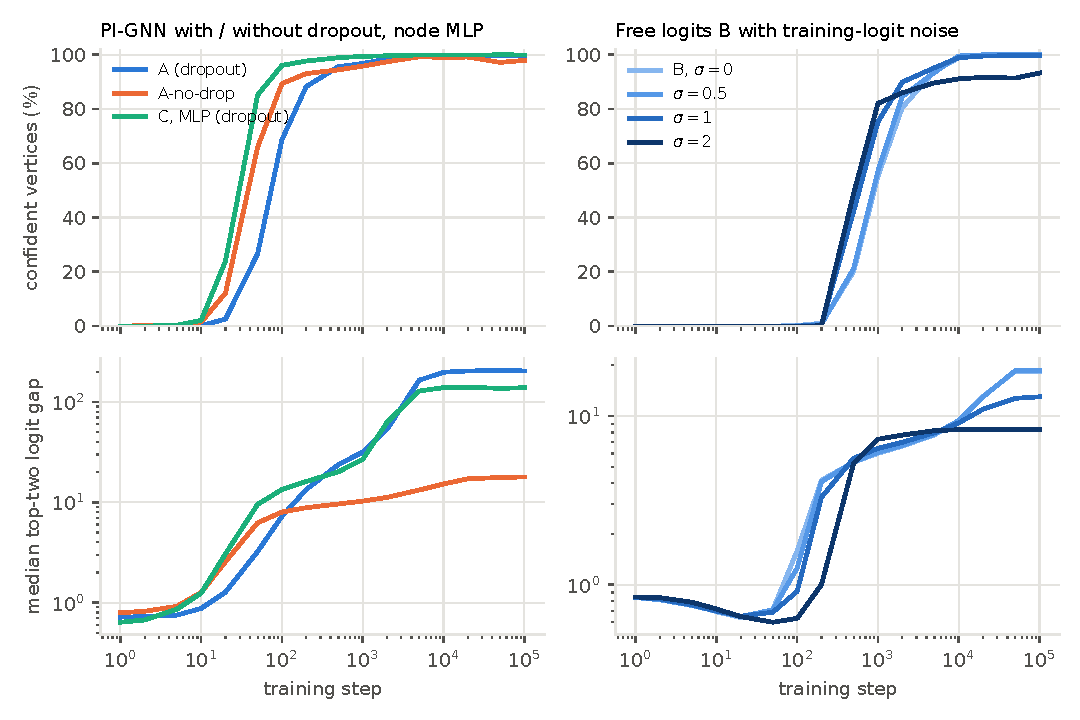
\includegraphics[width=\textwidth]{appendix/figures/confidence.pdf}
\caption{Output confidence over training: median over 68 graphs of 5-seed means. Top: share of
vertices with $p_{\max}\ge0.99$. Bottom: median top-two logit gap (log scale).}
\label{fig:conf}
\end{figure}

\begin{table}[h]
\centering\small
% generated by scripts/make_appendix.py -- do not edit by hand
\begin{tabular}{@{}lrrrrrrrrrr@{}}
\toprule
& \multicolumn{5}{c}{confident vertices, $p_{\max}\ge0.99$ (\%)} & \multicolumn{5}{c}{median top-two logit gap} \\
\cmidrule(lr){2-6}\cmidrule(l){7-11}
step & 10 & $10^2$ & $10^3$ & $10^4$ & $10^5$ & 10 & $10^2$ & $10^3$ & $10^4$ & $10^5$ \\
\midrule
A (PI-GNN) & 0.2 & 68.7 & 96.7 & 99.6 & 99.6 & 0.9 & 7.3 & 31.7 & 197.7 & 203.7 \\
A-no-drop & 1.5 & 89.3 & 95.8 & 99.0 & 97.9 & 1.3 & 8.0 & 10.3 & 15.2 & 17.9 \\
C (MLP) & 2.1 & 96.0 & 99.4 & 99.8 & 99.9 & 1.2 & 13.4 & 26.8 & 138.9 & 138.5 \\
B & 0.0 & 0.2 & 55.2 & 98.8 & 100.0 & 0.7 & 1.6 & 6.0 & 9.4 & 18.4 \\
B-noise-0.5 & 0.0 & 0.1 & 57.1 & 99.5 & 100.0 & 0.7 & 1.3 & 6.1 & 9.4 & 18.6 \\
B-noise-1 & 0.0 & 0.0 & 75.3 & 98.9 & 99.7 & 0.7 & 0.9 & 6.4 & 9.1 & 13.0 \\
B-noise-2 & 0.0 & 0.0 & 82.0 & 91.1 & 93.2 & 0.7 & 0.6 & 7.3 & 8.3 & 8.3 \\
\bottomrule
\end{tabular}

\caption{Confidence at selected steps (medians over graphs of seed means).}
\label{tab:conf}
\end{table}

\begin{table}[h]
\centering\small
% generated by scripts/make_appendix.py -- do not edit by hand
\begin{tabular}{@{}lccc@{}}
\toprule
difference in confident vertices (points) & step $10^2$ & step $10^3$ & step $10^5$ \\
\midrule
A-no-drop $-$ A & $+15.2$ [$+8.6$, $+20.4$] & $-0.8$ [$-2.6$, $-0.4$] & $-1.0$ [$-1.7$, $-0.5$] \\
C $-$ A & $+20.3$ [$+14.6$, $+32.2$] & $+1.9$ [$+0.8$, $+4.4$] & $+0.0$ [$+0.0$, $+0.1$] \\
B-noise-0.5 $-$ B & $-0.1$ [$-0.3$, $+0.0$] & $+2.9$ [$+1.4$, $+4.0$] & $+0.0$ [$+0.0$, $+0.0$] \\
B-noise-1 $-$ B & $-0.2$ [$-0.7$, $+0.0$] & $+11.9$ [$+8.7$, $+14.9$] & $-0.2$ [$-0.3$, $-0.2$] \\
B-noise-2 $-$ B & $-0.2$ [$-0.8$, $+0.0$] & $+19.1$ [$+11.8$, $+23.0$] & $-6.5$ [$-12.1$, $-2.6$] \\
\bottomrule
\end{tabular}

\caption{Paired per-graph difference in the share of confident vertices (percentage points), median
over graphs with 95\% bootstrap CI.}
\label{tab:confdiff}
\end{table}

\section{RQ3: soft output or decoder?}
\label{sec:rq3}

\begin{table}[h]
\centering\small
\resizebox{\textwidth}{!}{% generated by scripts/make_appendix.py -- do not edit by hand
\begin{tabular}{@{}lccccr@{}}
\toprule
Comparison (first vs.\ second) & W/T/L & median $d$ & 95\% CI & mean $C$, first / second & $p$ \\
\midrule
D-CE vs.\ argmax (trained $P$), raw & 33/35/0 & $-11.4\%$ & [$-31.0\%$, $-5.0\%$] & 125.1 / 1517.3 & $1.6{\times}10^{-10}$ \\
D-CE vs.\ argmax (trained $P$), desc. & 22/46/0 & $-2.8\%$ & [$-5.4\%$, $-0.2\%$] & 111.4 / 114.9 & $1.1{\times}10^{-6}$ \\
trained vs.\ near-uniform (D-CE), raw & 26/26/16 & $-7.3\%$ & [$-21.3\%$, $0.0\%$] & 125.1 / 161.2 & 0.304 \\
trained vs.\ near-uniform (D-CE), desc. & 27/28/13 & $0.0\%$ & [$-7.2\%$, $0.0\%$] & 111.4 / 121.1 & 0.227 \\
trained vs.\ colour-scrambled (D-CE), raw & 65/3/0 & $-61.8\%$ & [$-67.9\%$, $-48.3\%$] & 125.1 / 209.1 & $1.0{\times}10^{-12}$ \\
trained vs.\ colour-scrambled (D-CE), desc. & 48/20/0 & $-25.5\%$ & [$-34.3\%$, $-19.0\%$] & 111.4 / 127.0 & $2.4{\times}10^{-12}$ \\
\midrule
trained vs.\ vertex-shuffled (D-CE), raw & 66/2/0 & $-59.8\%$ & [$-65.6\%$, $-47.2\%$] & 125.1 / 205.5 & $8.0{\times}10^{-13}$ \\
trained vs.\ vertex-shuffled (D-CE), desc. & 56/12/0 & $-29.9\%$ & [$-41.8\%$, $-22.8\%$] & 111.4 / 128.5 & $1.6{\times}10^{-12}$ \\
trained vs.\ untrained (D-CE), raw & 61/6/1 & $-54.5\%$ & [$-65.8\%$, $-50.2\%$] & 125.1 / 202.6 & $3.9{\times}10^{-11}$ \\
trained vs.\ untrained (D-CE), desc. & 51/14/3 & $-22.2\%$ & [$-31.4\%$, $-16.8\%$] & 111.4 / 127.6 & $1.4{\times}10^{-8}$ \\
near-uniform vs.\ colour-scrambled (D-CE), raw & 66/2/0 & $-55.4\%$ & [$-70.6\%$, $-33.5\%$] & 161.2 / 209.1 & $7.6{\times}10^{-13}$ \\
near-uniform vs.\ colour-scrambled (D-CE), desc. & 41/24/3 & $-17.5\%$ & [$-37.5\%$, $-10.6\%$] & 121.1 / 127.0 & $4.8{\times}10^{-11}$ \\
D-CE vs.\ argmax (near-uniform $P$), raw & 68/0/0 & $-92.6\%$ & [$-97.5\%$, $-79.7\%$] & 161.2 / 550.2 & $7.6{\times}10^{-13}$ \\ % new: not in exp2_summary.csv
D-CE vs.\ argmax (near-uniform $P$), desc. & 57/9/2 & $-43.1\%$ & [$-61.7\%$, $-20.3\%$] & 121.1 / 135.4 & $4.1{\times}10^{-12}$ \\ % new: not in exp2_summary.csv
trained vs.\ near-uniform (argmax), raw & 64/0/4 & $-86.9\%$ & [$-91.7\%$, $-80.7\%$] & 1517.3 / 550.2 & $3.0{\times}10^{-8}$ \\
trained vs.\ near-uniform (argmax), desc. & 60/7/1 & $-40.6\%$ & [$-50.3\%$, $-27.7\%$] & 114.9 / 135.4 & $1.5{\times}10^{-12}$ \\
trained vs.\ colour-scrambled (argmax), raw & 64/0/4 & $-87.3\%$ & [$-92.1\%$, $-80.4\%$] & 1517.3 / 552.3 & $3.0{\times}10^{-8}$ \\
trained vs.\ colour-scrambled (argmax), desc. & 60/7/1 & $-40.1\%$ & [$-50.2\%$, $-29.1\%$] & 114.9 / 134.5 & $1.8{\times}10^{-12}$ \\
saturation vs.\ random order (D-CE), raw & 3/63/2 & $0.0\%$ & [$-0.2\%$, $0.0\%$] & 125.1 / 125.2 & 0.116 \\
saturation vs.\ random order (D-CE), desc. & 4/64/0 & $0.0\%$ & [$0.0\%$, $0.0\%$] & 111.4 / 112.8 & 0.162 \\
best of 32 samples vs.\ argmax, raw & 4/64/0 & $0.0\%$ & [$0.0\%$, $0.0\%$] & 193.5 / 1517.3 & $3.1{\times}10^{-5}$ \\
best of 32 samples vs.\ argmax, desc. & 2/65/1 & $0.0\%$ & [$0.0\%$, $0.0\%$] & 113.3 / 114.9 & 0.008 \\
\bottomrule
\end{tabular}
}
\caption{All RQ3 comparisons on A's frozen $10^5$-step outputs (68 graphs, 5 seeds), raw and after
strict descent. Rows above the rule are the three pre-registered primary comparisons. ``D-CE vs.\
argmax (near-uniform $P$)'' is new in this appendix and supports the first paragraph of Section~4.3.
Sampling rows compare the best of 32 samples.}
\label{tab:rq3all}
\end{table}

\begin{table}[h]
\centering\small
% generated by scripts/make_appendix.py -- do not edit by hand
\begin{tabular}{@{}lrcrccr@{}}
\toprule
& & \multicolumn{3}{c}{trained vs.\ near-uniform (D-CE + desc.)} & \multicolumn{2}{c}{D-CE vs.\ argmax (+ desc.)} \\
\cmidrule(lr){3-5}\cmidrule(l){6-7}
family & graphs & W/T/L & median $d$ & mean $C$ & W/T/L & median $d$ \\
\midrule
Queen & 12 & 12/0/0 & $-18.5\%$ & 29.53 / 35.65 & 1/11/0 & $-1.3\%$ \\
DSJC & 4 & 3/1/0 & $-16.1\%$ & 32.70 / 39.05 & 2/2/0 & $-3.5\%$ \\
School & 2 & 2/0/0 & $-13.0\%$ & 350.50 / 400.50 & 2/0/0 & $-9.9\%$ \\
Flat & 5 & 3/2/0 & $-5.1\%$ & 644.32 / 668.96 & 1/4/0 & $-2.7\%$ \\
Leighton & 12 & 7/0/5 & $-7.1\%$ & 255.05 / 286.13 & 5/7/0 & $-4.5\%$ \\
DSJR & 3 & 0/1/2 & $+44.0\%$ & 17.93 / 12.33 & 2/1/0 & $-31.9\%$ \\
fpsol & 3 & 0/2/1 & $+57.1\%$ & 2.13 / 1.13 & 3/0/0 & $-42.3\%$ \\
inithx & 3 & 0/1/2 & $+140.0\%$ & 2.60 / 1.00 & 3/0/0 & $-41.9\%$ \\
Miles & 5 & 0/2/3 & $+100.0\%$ & 2.32 / 1.08 & 2/3/0 & $-10.0\%$ \\
zeroin & 3 & 0/3/0 & $+20.0\%$ & 1.20 / 1.00 & 1/2/0 & $-37.5\%$ \\
mulsol & 5 & 0/5/0 & $0.0\%$ & 1.68 / 1.60 & 0/5/0 & $0.0\%$ \\
Mycielski & 5 & 0/5/0 & $0.0\%$ & 1.04 / 1.08 & 0/5/0 & $0.0\%$ \\
Social (book) & 5 & 0/5/0 & $0.0\%$ & 1.12 / 1.08 & 0/5/0 & $0.0\%$ \\
games120 & 1 & 0/1/0 & $0.0\%$ & 2.00 / 2.00 & 0/1/0 & $0.0\%$ \\
\bottomrule
\end{tabular}

\caption{RQ3 by family, after D-CE/argmax and descent. Negative $d$ favours trained $P$ (left) or
D-CE (right).}
\label{tab:rq3fam}
\end{table}

\begin{table}[h]
\centering\small
\resizebox{\textwidth}{!}{% generated by scripts/make_appendix.py -- do not edit by hand
\begin{tabular}{@{}lrrcccc@{}}
\toprule
& \multicolumn{2}{c}{mean $\Cd$} & \multicolumn{4}{c}{arm's D-CE + descent vs.\ \dots, W/T/L (median $d$)} \\
\cmidrule(lr){2-3}\cmidrule(l){4-7}
arm & argmax & D-CE & own argmax + desc. & A, D-CE & near-uniform & own colour-scrambled \\
\midrule
A (PI-GNN) & 114.9 & 111.4 & 22/46/0 ($-2.8\%$) & -- & 27/28/13 ($0.0\%$) & 48/20/0 ($-25.5\%$) \\
A-no-drop & 115.7 & 117.0 & 10/48/10 ($-0.5\%$) & 4/34/30 ($+12.5\%$) & 9/36/23 ($+5.0\%$) & 44/22/2 ($-22.2\%$) \\
C (MLP) & 120.4 & 116.1 & 27/41/0 ($-6.2\%$) & 2/44/22 ($+4.7\%$) & 23/29/16 ($0.0\%$) & 47/21/0 ($-22.4\%$) \\
D (linearised) & 130.4 & 123.1 & 45/23/0 ($-14.6\%$) & 1/21/46 ($+20.0\%$) & 8/31/29 ($+6.8\%$) & 39/28/1 ($-11.5\%$) \\
B & 108.6 & 107.3 & 5/63/0 ($-0.8\%$) & 14/24/30 ($+7.6\%$) & 25/17/26 ($0.0\%$) & 55/13/0 ($-27.2\%$) \\
B-rand & 107.1 & 106.2 & 5/63/0 ($-1.4\%$) & 14/25/29 ($+5.1\%$) & 26/15/27 ($0.0\%$) & 47/21/0 ($-20.5\%$) \\
B-noise-0.5 & 109.2 & 108.4 & 4/64/0 ($-0.4\%$) & 13/24/31 ($+4.1\%$) & 26/17/25 ($0.0\%$) & 55/13/0 ($-27.5\%$) \\
B-noise-1 & 92.5 & 92.3 & 1/67/0 ($0.0\%$) & 31/30/7 ($-12.9\%$) & 36/25/7 ($-16.7\%$) & 56/12/0 ($-44.0\%$) \\
B-noise-2 & 83.4 & 83.4 & 0/68/0 ($0.0\%$) & 35/29/4 ($-18.7\%$) & 36/27/5 ($-21.2\%$) & 58/10/0 ($-58.0\%$) \\
\bottomrule
\end{tabular}
}
\caption{D-CE applied to every RQ2 arm (after descent). Negative $d$ favours the arm's D-CE output.
The near-uniform reference is shared across arms because it depends only on the graph, $k$ and seed.
Across all nine arms, the median over graphs of the relative range
$(\max_a\bar C_a-\min_a\bar C_a)/\mathrm{mean}_a\bar C_a$ falls from 0.865 with argmax + descent to
0.685 with D-CE + descent; within graphs it shrinks on 44, ties on 16 and grows on 8 (median
$-10.2\%$).}
\label{tab:rq3arms}
\end{table}

\begin{table}[h]
\centering\small
% generated by scripts/make_appendix.py -- do not edit by hand
\begin{tabular}{@{}lrrrr@{}}
\toprule
& \multicolumn{3}{c}{trained $P$, 340 runs (s)} & all five A inputs (s) \\
\cmidrule(lr){2-4}
decoder + strict descent & decode & descent & total & total \\
\midrule
argmax & 0.44 & 29.94 & 30.39 & 348.6 \\
D-CE (saturation order) & 11.49 & 9.83 & 21.32 & 140.7 \\
D-CE (random order) & 6.17 & 8.73 & 14.90 & 115.3 \\
best of 32 samples & 0.54 & 788.80 & 789.34 & 10{,}475.1 \\
\bottomrule
\end{tabular}

\caption{Summed decoder and descent time (CPU, seconds) over A's 340 runs. Best-of-32 sampling is
$26\times$ the cost of argmax + descent; D-CE + descent is cheaper than argmax + descent because its
starts need less repair.}
\label{tab:rq3cost}
\end{table}

\clearpage
\section{Per-graph results}
\label{sec:pergraph}

{\footnotesize\setlength{\tabcolsep}{3.5pt}
% generated by scripts/make_appendix.py -- do not edit by hand
\begin{longtable}{@{}llrrrrrrrrrrr@{}}
\caption{Per-graph results at $10^5$ steps: mean conflicts over 5 seeds (TabuCol: 10 seeds, time-matched to
PI-GNN). A raw / desc.: PI-GNN argmax before / after strict descent. B, B-noise-2: after descent (identical to
raw, all runs are SFO). DSATUR: fixed-$k$ DSATUR + descent. D-CE: D-CE + descent on A's trained $P$ and on the
near-uniform (graph-only) input.}\label{tab:pergraph}\\
\toprule
graph & family & $n$ & $m$ & $k$ & A raw & A desc. & B & B-n-2 & DSATUR & TabuCol & D-CE tr. & D-CE unif. \\
\midrule\endfirsthead
\toprule
graph & family & $n$ & $m$ & $k$ & A raw & A desc. & B & B-n-2 & DSATUR & TabuCol & D-CE tr. & D-CE unif. \\
\midrule\endhead
\bottomrule\endfoot
queen10\_10 & Queen & 100 & 1470 & 10 & 18.4 & 18.4 & 22.4 & 13.0 & 26.6 & 4.4 & 18.2 & 24.0 \\
queen11\_11 & Queen & 121 & 1980 & 10 & 38.2 & 37.8 & 43.6 & 33.4 & 48.2 & 26.4 & 37.2 & 50.2 \\
queen12\_12 & Queen & 144 & 2596 & 11 & 47.6 & 47.2 & 49.2 & 36.2 & 54.0 & 30.1 & 46.8 & 54.6 \\
queen13\_13 & Queen & 169 & 3328 & 12 & 53.4 & 53.4 & 57.6 & 40.2 & 52.4 & 33.4 & 52.4 & 59.2 \\
queen14\_14 & Queen & 196 & 4186 & 13 & 62.4 & 62.2 & 62.6 & 42.6 & 64.4 & 36.1 & 60.4 & 67.0 \\
queen15\_15 & Queen & 225 & 5180 & 14 & 71.8 & 71.0 & 67.0 & 45.8 & 66.8 & 39.6 & 66.6 & 71.8 \\
queen5\_5 & Queen & 25 & 160 & 4 & 13.0 & 13.0 & 13.6 & 12.8 & 13.0 & 12.0 & 13.0 & 15.2 \\
queen6\_6 & Queen & 36 & 290 & 6 & 6.4 & 6.4 & 8.6 & 5.4 & 9.0 & 4.0 & 6.4 & 8.8 \\
queen7\_7 & Queen & 49 & 476 & 6 & 19.4 & 19.4 & 22.8 & 18.8 & 22.0 & 16.0 & 19.4 & 23.2 \\
queen8\_12 & Queen & 96 & 1368 & 11 & 11.6 & 11.2 & 12.4 & 8.0 & 13.8 & 8.0 & 10.8 & 13.6 \\
queen8\_8 & Queen & 64 & 728 & 8 & 11.0 & 11.0 & 12.8 & 9.6 & 20.0 & 2.0 & 10.4 & 17.8 \\
queen9\_9 & Queen & 81 & 1056 & 9 & 12.8 & 12.8 & 18.2 & 10.0 & 21.0 & 3.0 & 12.8 & 22.4 \\
DSJC125.1 & DSJC & 125 & 736 & 4 & 28.0 & 28.0 & 39.2 & 32.4 & 39.0 & 19.0 & 28.0 & 45.2 \\
DSJC125.5 & DSJC & 125 & 3891 & 16 & 32.0 & 31.6 & 27.4 & 12.2 & 34.6 & 5.0 & 29.4 & 35.6 \\
DSJC125.9 & DSJC & 125 & 6961 & 43 & 40.4 & 15.8 & 13.4 & 2.2 & 16.2 & 1.0 & 16.2 & 19.0 \\
DSJC250.9 & DSJC & 250 & 27897 & 71 & 4{,}968 & 62.8 & 37.0 & 9.6 & 51.4 & 1.0 & 57.2 & 56.4 \\
school1 & School & 385 & 19095 & 13 & 502.6 & 465.8 & 274.8 & 130.2 & 270.6 & 126.0 & 404.8 & 439.0 \\
school1\_nsh & School & 352 & 14612 & 13 & 340.8 & 317.8 & 249.2 & 147.2 & 367.6 & 80.0 & 296.2 & 362.0 \\
flat1000\_50\_0 & Flat & 1000 & 245000 & 49 & 3{,}367 & 1{,}540 & 1{,}464 & 1{,}219 & 1{,}590 & 1{,}148 & 1{,}537 & 1{,}592 \\
flat1000\_60\_0 & Flat & 1000 & 245830 & 59 & 2{,}492 & 1{,}019 & 929.4 & 718.2 & 1{,}025 & 618.9 & 1{,}039 & 1{,}054 \\
flat300\_20\_0 & Flat & 300 & 21375 & 19 & 374.0 & 354.2 & 315.6 & 256.6 & 366.8 & 50.0 & 344.6 & 363.0 \\
flat300\_26\_0 & Flat & 300 & 21633 & 25 & 205.8 & 180.6 & 159.0 & 106.4 & 193.6 & 75.3 & 173.8 & 187.4 \\
flat300\_28\_0 & Flat & 300 & 21695 & 27 & 163.8 & 134.2 & 116.4 & 72.4 & 134.0 & 46.5 & 127.4 & 148.2 \\
le450\_15a & Leighton & 450 & 8168 & 14 & 72.8 & 71.6 & 69.0 & 36.0 & 50.4 & 21.0 & 68.0 & 57.6 \\
le450\_15b & Leighton & 450 & 8169 & 14 & 75.0 & 73.0 & 69.6 & 36.2 & 48.0 & 21.7 & 66.8 & 51.6 \\
le450\_15c & Leighton & 450 & 16680 & 14 & 333.8 & 322.4 & 312.4 & 234.0 & 329.2 & 93.0 & 314.4 & 346.6 \\
le450\_15d & Leighton & 450 & 16750 & 14 & 343.2 & 336.2 & 309.0 & 244.4 & 351.8 & 95.7 & 322.2 & 352.2 \\
le450\_25a & Leighton & 450 & 8260 & 24 & 16.8 & 15.8 & 16.6 & 8.6 & 11.0 & 6.0 & 14.4 & 13.0 \\
le450\_25b & Leighton & 450 & 8263 & 24 & 14.8 & 12.4 & 15.0 & 7.4 & 12.0 & 6.0 & 11.8 & 12.8 \\
le450\_25c & Leighton & 450 & 17343 & 24 & 122.0 & 109.0 & 87.2 & 39.6 & 62.8 & 21.5 & 96.6 & 77.6 \\
le450\_25d & Leighton & 450 & 17425 & 24 & 116.6 & 104.6 & 86.2 & 39.2 & 63.4 & 20.3 & 93.4 & 77.2 \\
le450\_5a & Leighton & 450 & 5714 & 4 & 508.0 & 508.0 & 552.8 & 434.6 & 651.4 & 407.7 & 507.4 & 646.4 \\
le450\_5b & Leighton & 450 & 5734 & 4 & 541.6 & 540.0 & 567.8 & 472.4 & 664.4 & 412.0 & 539.0 & 640.8 \\
le450\_5c & Leighton & 450 & 9803 & 4 & 518.8 & 518.6 & 544.8 & 546.0 & 734.0 & 489.0 & 515.0 & 549.8 \\
le450\_5d & Leighton & 450 & 9757 & 4 & 511.6 & 511.6 & 546.6 & 519.2 & 746.4 & 479.1 & 511.6 & 608.0 \\
DSJR500.1 & DSJR & 500 & 3555 & 11 & 7.6 & 7.6 & 13.8 & 4.4 & 4.0 & 4.9 & 7.2 & 5.0 \\
DSJR500.1c & DSJR & 500 & 121275 & 84 & 39{,}210 & 40.8 & 25.0 & 4.4 & 12.6 & 3.8 & 27.8 & 14.0 \\
DSJR500.5 & DSJR & 500 & 58862 & 121 & 47{,}161 & 59.4 & 50.2 & 12.6 & 12.0 & 9.4 & 18.8 & 18.0 \\
fpsol2.i.1 & fpsol & 496 & 11654 & 64 & 34.2 & 2.4 & 5.2 & 1.2 & 1.0 & 14.0 & 1.2 & 1.0 \\
fpsol2.i.2 & fpsol & 451 & 8691 & 29 & 11.0 & 5.2 & 7.4 & 3.8 & 1.0 & 30.9 & 3.0 & 1.0 \\
fpsol2.i.3 & fpsol & 425 & 8688 & 29 & 6.6 & 3.8 & 6.8 & 2.6 & 1.0 & 36.5 & 2.2 & 1.4 \\
inithx.i.1 & inithx & 864 & 18707 & 53 & 24.4 & 3.0 & 8.6 & 6.0 & 1.0 & 27.5 & 1.8 & 1.0 \\
inithx.i.2 & inithx & 645 & 13979 & 30 & 14.2 & 6.2 & 11.2 & 4.2 & 1.0 & 56.9 & 3.6 & 1.0 \\
inithx.i.3 & inithx & 621 & 13969 & 30 & 10.0 & 4.6 & 10.8 & 4.4 & 1.0 & 53.3 & 2.4 & 1.0 \\
miles1000 & Miles & 128 & 3216 & 41 & 17.6 & 4.4 & 3.4 & 1.2 & 1.0 & 1.1 & 3.4 & 1.0 \\
miles1500 & Miles & 128 & 5198 & 72 & 526.8 & 3.8 & 1.8 & 1.0 & 1.0 & 1.0 & 2.0 & 1.0 \\
miles250 & Miles & 128 & 387 & 7 & 1.4 & 1.2 & 2.0 & 1.4 & 1.0 & 1.0 & 1.2 & 1.0 \\
miles500 & Miles & 128 & 1170 & 19 & 2.6 & 2.0 & 2.0 & 1.0 & 1.0 & 1.1 & 1.8 & 1.2 \\
miles750 & Miles & 128 & 2113 & 30 & 8.0 & 2.8 & 3.4 & 1.2 & 1.0 & 1.2 & 3.2 & 1.2 \\
zeroin.i.1 & zeroin & 211 & 4100 & 48 & 20.0 & 1.6 & 2.0 & 1.0 & 1.0 & 7.2 & 1.0 & 1.0 \\
zeroin.i.2 & zeroin & 211 & 3541 & 29 & 5.6 & 2.2 & 4.0 & 1.0 & 1.0 & 8.8 & 1.2 & 1.0 \\
zeroin.i.3 & zeroin & 206 & 3540 & 29 & 5.6 & 2.0 & 2.8 & 1.0 & 1.0 & 8.7 & 1.4 & 1.0 \\
mulsol.i.1 & mulsol & 197 & 3925 & 48 & 23.8 & 1.0 & 1.8 & 1.0 & 1.0 & 2.3 & 1.2 & 1.0 \\
mulsol.i.2 & mulsol & 188 & 3885 & 30 & 5.0 & 2.0 & 3.8 & 2.0 & 2.0 & 12.3 & 2.0 & 2.0 \\
mulsol.i.3 & mulsol & 184 & 3916 & 30 & 3.8 & 2.0 & 3.8 & 2.0 & 2.0 & 13.0 & 2.0 & 2.0 \\
mulsol.i.4 & mulsol & 185 & 3946 & 30 & 3.4 & 2.0 & 4.4 & 2.0 & 2.0 & 12.2 & 2.0 & 2.0 \\
mulsol.i.5 & mulsol & 186 & 3973 & 30 & 4.8 & 1.4 & 3.6 & 1.0 & 1.0 & 12.6 & 1.2 & 1.0 \\
myciel3 & Mycielski & 11 & 20 & 3 & 1.0 & 1.0 & 1.0 & 1.0 & 1.0 & 1.0 & 1.0 & 1.0 \\
myciel4 & Mycielski & 23 & 71 & 4 & 1.0 & 1.0 & 1.0 & 1.0 & 1.0 & 1.0 & 1.0 & 1.0 \\
myciel5 & Mycielski & 47 & 236 & 5 & 1.2 & 1.0 & 1.0 & 1.0 & 1.0 & 1.0 & 1.0 & 1.0 \\
myciel6 & Mycielski & 95 & 755 & 6 & 2.0 & 1.0 & 1.4 & 1.0 & 1.0 & 1.0 & 1.2 & 1.2 \\
myciel7 & Mycielski & 191 & 2360 & 7 & 1.8 & 1.0 & 1.0 & 1.0 & 1.0 & 1.0 & 1.0 & 1.2 \\
anna & Social (book) & 138 & 493 & 10 & 1.8 & 1.0 & 1.6 & 1.0 & 1.0 & 1.0 & 1.0 & 1.0 \\
david & Social (book) & 87 & 406 & 10 & 1.0 & 1.0 & 1.6 & 1.0 & 1.0 & 1.0 & 1.0 & 1.0 \\
homer & Social (book) & 561 & 1628 & 12 & 2.0 & 2.0 & 2.4 & 1.0 & 1.0 & 1.1 & 1.6 & 1.0 \\
huck & Social (book) & 74 & 301 & 10 & 1.4 & 1.0 & 1.2 & 1.0 & 1.0 & 1.0 & 1.0 & 1.0 \\
jean & Social (book) & 80 & 254 & 9 & 1.0 & 1.0 & 1.0 & 1.0 & 1.0 & 1.0 & 1.0 & 1.4 \\
games120 & games120 & 120 & 638 & 8 & 2.0 & 2.0 & 2.0 & 2.0 & 2.0 & 2.0 & 2.0 & 2.0 \\
\end{longtable}
}

\section{Further efforts: domain knowledge from a convex relaxation}
\label{sec:sdp}

\paragraph{Motivation.} The Potts loss has no relaxation gap: its continuous minimum equals the
discrete one \citep{rosenberg1972}, so descending it adds no information beyond what local moves can
find. Colouring has a classical relaxation that does carry global information, vector colouring by
semidefinite programming \citep{karger1998sdp}. We use the Frieze--Jerrum form at $k$ colours
\citep{frieze1997maxkcut}: unit vectors $v_i$ whose pairwise inner products are at least $-1/(k-1)$,
the value between the vertices of a regular simplex, maximising $\sum_{\{u,v\}\in E}(1-v_u^{\top}v_v)$.
A proper $k$-colouring placed on the simplex puts every edge exactly at this floor. The problem is
convex; we solve it approximately with a rank-32 Burer--Monteiro factorisation
\citep{burer2003nonlinear}, in 11--132\,s per graph on one CPU.

\paragraph{Two uses.} (i)~As domain-informed input to PI-GNN: the vectors initialise its vertex
embeddings (\emph{FJ init}). (ii)~Alone: k-means on the vectors gives a colouring, which can also seed
TabuCol. We ran both on the 12 harder DIMACS graphs of the main paper's second protocol (Section~3
there; 2 seeds), against PI-GNN with the best setting of a small pilot, DSATUR and TabuCol
(Table~\ref{tab:sdp}).

\begin{table}[h]
\centering\small
\begin{tabular}{@{}lrrrrr@{}}
\toprule
graph ($k$) & PI-GNN & +FJ init & SDP alone & DSATUR & TabuCol \\
\midrule
DSJC125.5 (17) & 19 & 10 & 31 & 21 & 0 \\
DSJC250.5 (28) & 55.5 & 42 & 50 & 60 & 0.6 \\
flat300\_28\_0 (28) & 110 & 96 & 153 & 124 & 32.2 \\
le450\_15a (15) & 31 & 36.5 & 256 & 7 & 0 \\
le450\_15b (15) & 35 & 32.5 & 238 & 7 & 0 \\
le450\_15c (15) & 223 & \textbf{0} & 2 & 248 & 16.2 \\
le450\_15d (15) & 215.5 & \textbf{0.5} & 8 & 250 & 26.8 \\
queen10\_10 (11) & 10 & 9.5 & 54 & 10 & 0 \\
queen12\_12 (12) & 31 & 26 & 61 & 29 & 9.6 \\
queen14\_14 (14) & 32.5 & 32 & 91 & 32 & 13.4 \\
queen15\_15 (15) & 41.5 & 36 & 94 & 42 & 15.2 \\
queen16\_16 (16) & 43.5 & 46 & 117 & 44 & 17 \\
\bottomrule
\end{tabular}
\caption{Conflicts at $k$ colours (second protocol, mean of 2 seeds). PI-GNN and +FJ init: best
colouring found during training; SDP alone: k-means on the FJ vectors, best of 5; DSATUR: best of 11
randomised runs; TabuCol: 10\,s, mean of 5 runs.}
\label{tab:sdp}
\end{table}

\paragraph{Where structure is global, geometry wins.} FJ init improves PI-GNN on 10 of the 12 graphs.
On the Leighton graphs le450\_15c/d, built around a planted 15-colouring \citep{leighton1979}, it is
decisive: 0 and 0.5 conflicts, where plain PI-GNN keeps over 200 and TabuCol 16--27 after 10\,s
(7--24 after 60\,s). The control shows why. 95--97\% of edges sit exactly at the floor, so the SDP has
recovered the planted colouring, and TabuCol started from its k-means colouring finds a proper
colouring within 1--72 iterations (10 of 10 starts). The network is not needed: the geometry carries
the solution.

\paragraph{Elsewhere it does not.} On random, queen and the sparser Leighton graphs (le450\_15a/b),
the vectors alone are worse than DSATUR on 9 of 10 graphs (e.g.\ 54 vs.\ 10 conflicts on
queen10\_10), FJ init helps PI-GNN unevenly (most on DSJC125.5, from 19 to 10), and TabuCol stays far
ahead. Earlier small-scale tests agree. In an RLF-style colour-class extraction on 13 small graphs,
SDP vectors lowered the mean excess over the best known colour count from 0.615 (RLF) to 0.385, but
random unit vectors in the same procedure reached 0.462 (3/35/1 SDP vs.\ random). As PI-GNN input
features on 9 small graphs, FJ vectors beat the same rows shuffled (21/3/3) but not identity features
significantly (16/6/5, Holm-corrected $p=0.18$).

\paragraph{Insight.} Domain knowledge from a convex relaxation helps exactly where an instance hides
global structure. There it solves what neither PI-GNN nor TabuCol can, and the Potts loss, being
exact, cannot supply it. Where hardness lies in a rugged landscape instead, only search helps.
Testing all twelve Leighton graphs and planted-partition models would locate the boundary.

\bibliographystyle{acl_natbib}
\bibliography{custom}

\end{document}
